\documentclass[../../main.tex]{subfiles}
\begin{document}

\begin{flushright}
\footnotesize\textit{【自動文字起こし・要確認】}
\end{flushright}

{\bf [解]}
$|BD|=x$ とする．$\angle CBD=\theta$ とする．この時題意から $\angle ACB=2\theta$ である．$|CD|=y$ とする．まず，$\triangle ABC$ の成立条件から
\begin{align}
0<2\theta<\dfrac{\pi}{2} \quad\therefore\ 0<\theta<\dfrac{\pi}{4} \quad \cdots \text{①}
\end{align}

\begin{figure}[htb]
\begin{center}
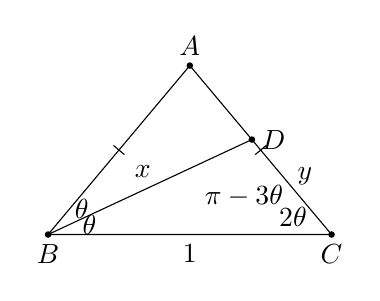
\begin{tikzpicture}[scale=3.6, >=stealth]
  % 二等辺三角形 ABC (底辺 BC=1, theta=25度として図示)
  \coordinate (B) at (0,0);
  \coordinate (C) at (1,0);
  \coordinate (A) at (0.5,0.596);
  % D: 角Bの二等分線 BD と辺 AC の交点 (角の二等分線定理から算出)
  \coordinate (D) at (0.719,0.335);
  \draw (B) -- (A) -- (C) -- cycle;
  \draw (B) -- (D);
  % AB=AC の印
  \draw (0.2308,0.3141) -- (0.2692,0.2819);
  \draw (0.7692,0.3141) -- (0.7308,0.2819);
  \fill (B) circle (0.33pt) node[below] {$B$};
  \fill (C) circle (0.33pt) node[below] {$C$};
  \fill (A) circle (0.33pt) node[above] {$A$};
  \fill (D) circle (0.33pt) node[right] {$D$};
  \node at (0.146,0.033) {$\theta$};
  \node[below] at (0.5,0) {$1$};
  \node at (0.119,0.091) {$\theta$};
  \node at (0.864,0.063) {$2\theta$};
  \node at (0.334,0.222) {$x$};
  \node at (0.906,0.206) {$y$};
  \node[below] at (0.691,0.208) {$\pi-3\theta$};
\end{tikzpicture}
\end{center}
\caption{$\triangle ABC$と点$D$の位置関係}
\end{figure}

$\triangle BCD$ に正弦定理を用いて，
\begin{align}
\dfrac{x}{\sin2\theta}=\dfrac{1}{\sin(\pi-3\theta)}=\dfrac{1}{\sin3\theta} \quad\therefore\ x=\dfrac{\sin2\theta}{\sin3\theta} \quad \cdots \text{②}
\end{align}
以下 $S=\sin\theta,\ C=\cos\theta$ とする．$\sin2\theta=2SC,\ \sin3\theta=3S-4S^3$ より，②から
\begin{align}
x=\dfrac{2SC}{3S-4S^3}=\dfrac{2C}{3-4S^2}=\dfrac{2C}{4C^2-1}
\end{align}
これは $C$ の単調減少関数であり，①とあわせて，
\begin{align}
\dfrac{2}{3}<x<\sqrt{2} \quad \left(\because\ \dfrac{2C}{4C^2-1}\xrightarrow{C\to\dfrac{\sqrt{2}}{2}+0}\sqrt{2},\quad \dfrac{2C}{4C^2-1}\xrightarrow{C\to1-0}\dfrac{2}{3}\right)
\end{align}


\newpage

\end{document}
